% Section 3: Other Repeated Games
%-------------------------------------------------------------------------------

\begin{frame}{A More Complicated Game}
  \begin{center}
  \begin{tabular}{cr|c|c|c|}
  	& \multicolumn{1}{c}{} & \multicolumn{3}{c}{Player 2}\\ \cline{3-5}
    \multicolumn{1}{c}{} & \multicolumn{1}{c}{} & x & y & z \\\cline{2-5}
    \multirow{3}*{Player 1}  & x & 5, 5 & 2, 7 & 1, 3 \\\cline{2-5}
                             & y & 7, 2 & 3, 3 & 0, 1 \\\cline{2-5}
                             & z & 3, 1 & 1, 0 & 2, 2 \\\cline{2-5}
  \end{tabular}
  \end{center}

  What are the \textbf{pure strategy Nash equilibria} of the \textit{one-shot} game?
\end{frame}

\begin{frame}{Repeated Game with 3 strategies per period}
  Now suppose that this game is played repeatedly an infinite number of times.  
  \begin{itemize}
    \item Can we do better than the single period equilibrium? 
  \end{itemize}
\end{frame}

\begin{frame}{Grim Trigger}
  \underline{Player 1} 
  \begin{align*}
    \begin{cases}
      t = 0 & \text{Play } x  \\ 
      t > 0 & 
      \begin{cases}
        \text{Play } x \text{ if only } x \text{ has been played } \\
        \text{Play } y \text{ if anything other than } x \text{has been played} \\
      \end{cases}
    \end{cases} 
  \end{align*}

  \underline{Player 2}
  \begin{itemize}
    \item $EV_{Coop} = \frac{5}{1-\delta}$ 
    \item $EV_{Cheat} = 7 + \frac{3\delta}{1-\delta}$
  \end{itemize}
\end{frame}

\begin{frame}{Grim Trigger}
  Solve for the value of $\delta$ for which this is a \textbf{SPNE}
  \vspace{50mm}
\end{frame}

\begin{frame}{Tit-for-Tat with extra forgiveness}
  \underline{Player 1} 
  \begin{align*}
    \begin{cases}
      t = 0 & \text{Play } x  \\ 
      t > 0 & \text{Play Player 2's strategy from } t-1 \\
       & 
      \begin{cases}
        \text{If P2 didn't play } x \text{ in } t-2 \text{ and P2 did play } x \text{ in } t-1, \\ 
        \text{ play P2's strategy from } t-1 \\ 
        \text{Else play } y \text{ forever} \\
      \end{cases}
    \end{cases} 
  \end{align*}

  \underline{Player 2}
  \begin{itemize}
    \item $EV_{Coop} = \frac{5}{1-\delta}$ 
    \item $EV_{Cheat} = 7 + 2\delta + \frac{5\delta^2}{1-\delta}$
  \end{itemize}
\end{frame}

\begin{frame}{Tit-for-Tat with extra forgiveness}
  Solve for the value of $\delta$ for which this is a \textbf{SPNE}
  \vspace{50mm}
\end{frame}

\begin{frame}{Tit-for-Tat vs Grim Trigger}
  Tit-for-Tat is more forgiving
  \begin{itemize}
    \item If $\delta \geq 1/2$, equilibrium is supported by Grim Trigger 
    \item If $\delta \geq 2/3$, equilibrium is supported by Tit-for-Tat
  \end{itemize}
\end{frame}

\begin{frame}{A reciprocating cooperation strategy}
    \underline{Player 1}
    $
      \begin{cases}
        t=0 & \text{Play } y \\ 
        t>0 & 
        \begin{cases}
          \text{Play } y \text{ if } t \text { is even } \\ 
          \text{Play } x \text{ if } t \text { is odd } \\ 
          \text{Play } z \text{ forever } \\
          \text{ if P2 played } y \\ 
          \text{ when $t$ is even} \\ 
        \end{cases}
      \end{cases} 
    $

    \underline{Player 2}
    $
      \begin{cases}
        t=0 & \text{Play } x \\ 
        t>0 & 
        \begin{cases}
          \text{Play } y \text{ if } t \text { is odd } \\ 
          \text{Play } x \text{ if } t \text { is even } \\ 
          \text{Play } z \text{ forever } \\
          \text{ if P2 played } y \\ 
          \text{ when $t$ is odd} \\ 
        \end{cases}
      \end{cases} 
      $
\end{frame}

\begin{frame}{A reciprocating cooperation strategy}
  Solve for the value of $\delta$ for which this is a \textbf{SPNE}
  \vspace{50mm}
\end{frame}

\begin{frame}{When can cooperation be achieved?}
  With all of these different ways of achieving repeated cooperation, 
  you might be wondering if there is a way to tell what strategies can actually work
\end{frame}

\begin{frame}{Folk Theorem}
  Any strategy is a potential SPNE for a \textbf{repeated} stage game if: 
  \begin{itemize}
    \item Both agents are sufficiently patient and far-sighted (high enough $\delta$)
    \item The payoffs from the cooperative strategy profile satisfy the two properties: 
    \begin{itemize}
      \item \textbf{Individually Rational:} the payoffs to each agent (weakly) exceed their minimax payoffs in the stage game 
      \item \textbf{Feasibility:} the payoffs are weighted averages of the payoffs found in the stage game
    \end{itemize}
  \end{itemize}
\end{frame}

\begin{frame}{Folk Theorem with 3x3 Repeated Game Example}
  \begin{center}
  \begin{tabular}{cr|c|c|c|}
  	& \multicolumn{1}{c}{} & \multicolumn{3}{c}{Player 2}\\ \cline{3-5}
    \multicolumn{1}{c}{} & \multicolumn{1}{c}{} & x & y & z \\\cline{2-5}
    \multirow{3}*{Player 1}  & x & 5, 5 & 2, 7 & 1, 3 \\\cline{2-5}
                             & y & 7, 2 & 3, 3 & 0, 1 \\\cline{2-5}
                             & z & 3, 1 & 1, 0 & 2, 2 \\\cline{2-5}
  \end{tabular}
  \end{center}

  The \alert{Minimax} equilibrium is (z,z)
  \begin{itemize}
    \item it \textit{minimizes} the \textit{maximum} payoff that your opponent could get
    \item The Minimax payoffs in this stage game are (2, 2)
    \item Intuitively, this is the \textit{safe} option: you can always fall back on it if cooperation fails
  \end{itemize}
\end{frame}

\begin{frame}{Folk Theorem with 3x3 Repeated Game Example payoffs}
  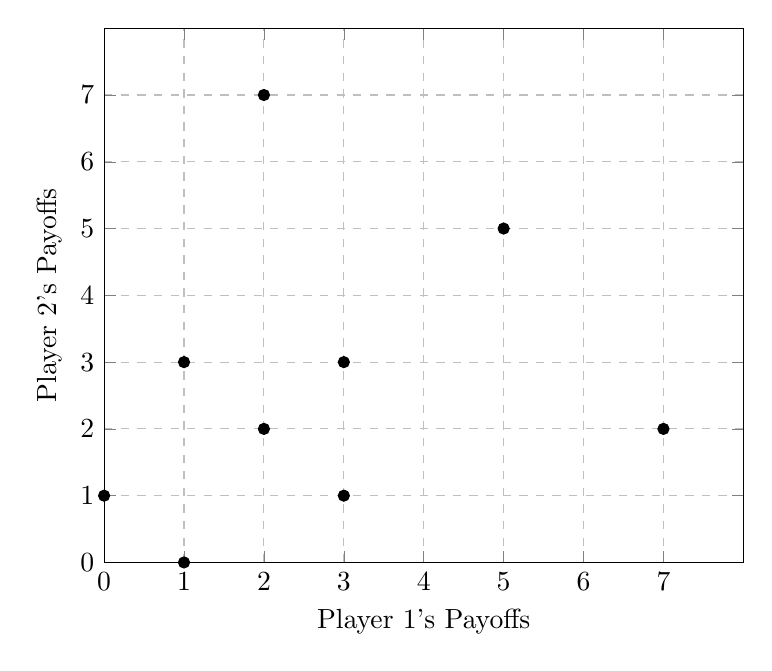
\begin{tikzpicture}
   \begin{axis}[
     width=0.8\textwidth,
     grid,
     xlabel={Player 1's Payoffs},
     ylabel={Player 2's Payoffs},
     xmin=0, xmax=8,
     ymin=0, ymax=8,
     xtick={0,1,...,7},
     ytick={0,1,...,7},
     grid style=dashed,
     ]
 
     \addplot[only marks]
     coordinates {
     (5,5) (2,7) (1,3) 
     (7,2) (3,3) (0,1)
     (3,1) (1,0) (2,2)
     };
   \end{axis}
 \end{tikzpicture}
\end{frame}

\begin{frame}{Folk Theorem with 3x3 Repeated Game Example}
  \begin{itemize}
    \item The shaded region of the graph shows us all of the strategy profiles which could be sustained by the \textbf{Folk Theorem} 
    \item This shows us why that strategy profile of alternating between (x, y) and (y, x) worked: 
    \begin{itemize}
      \item even though getting 2 on even or odd periods was no better than the Minimax payoffs, because you could alternate with the higher payoff of 7 you could do better as long as you are patient enough 
      \item this mix between (2, 7) and (7, 2) is \textit{within the convex hull} of sustainable payoffs
    \end{itemize}
  \end{itemize} 
\end{frame}

\begin{frame}{Cooperation in Repeated Games}
  \begin{itemize}
    \item As you can probably tell, there are an infinite number of strategy profiles which can achieve cooperation 
    \begin{itemize}
      \item We could allow for mixed strategies, which would work similar to the alternating example we saw 
      \item The Folk Theorem tells us that all we need is for all players to be patient enough 
      \item and also that the past plays are common knowledge
    \end{itemize}
  \end{itemize}
\end{frame}

\begin{frame}{Importance of the Folk Theorem}
  Why does this matter for real life? 
  \begin{itemize}
    \item Most strategic interactions in your life are repeated 
    \begin{itemize}
      \item Sharing chores with your roommates 
      \item Interacting in class with me every week
      \item Being nice to the barista at your regular cafe
    \end{itemize}
  \end{itemize}
\end{frame}

\begin{frame}{Importance of the Folk Theorem}
  \begin{itemize}
    \item Even when you don't repeatedly interact with the same exact people, you still see cooperative outcomes 
    \item \textbf{Institutions, Reputations, and Social Structures} all serve to allow for past interactions to be common knowledge
    \item The history of humanity is built on how we arrange our strategic interactions in ways so that people are incentivized to play nice with others
  \end{itemize}
\end{frame}

\begin{frame}{Importance of the Folk Theorem}
  Some caveats:
  \begin{itemize}
    \item People can't know exactly when the game will end; if they don't have any incentive from future cooperative gains, they will always defect
    \begin{itemize}
      \item Institutions have to \textit{seem} like they are infinitely lived (compared to finitely lived humans)
    \end{itemize}
    \item Cooperative equilibria must be better than peoples' outside options 
    \begin{itemize}
      \item If you make your institution too costly for people to engage with, they will opt out 
    \end{itemize}
    \item People need to be patient enough to make cooperation worth it
  \end{itemize}
\end{frame}
